\scanpage{22}
\mspage{21}
\figure{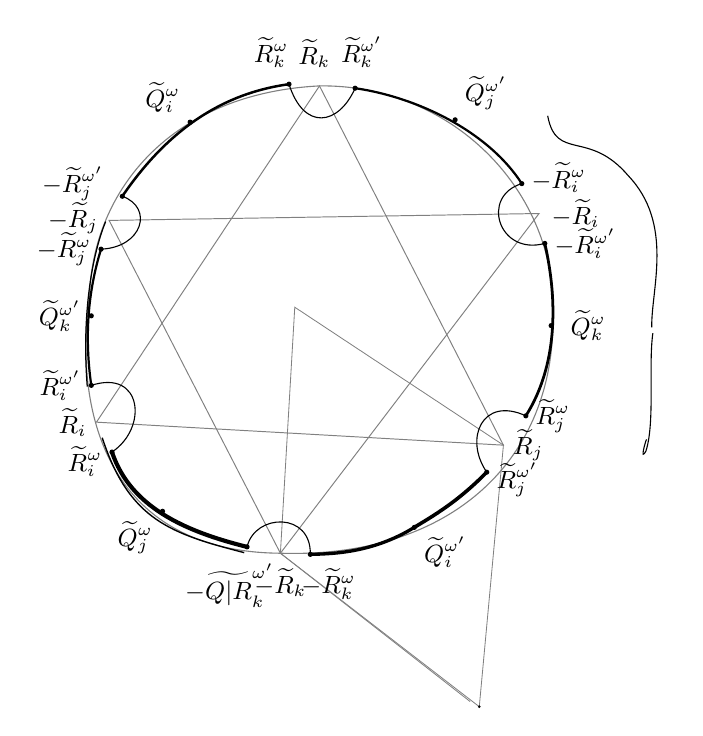
\begin{tikzpicture}[x=.73cm,y=.73cm,every node/.style={font=\small}]
\draw[gray,line width=.35pt] (2.22,7.01)--(9.7,7.13)--(5.2,1.22)--cycle;
\draw[gray,line width=.35pt] (5.88,9.35)--(2.0,3.5)--(9.08,3.1)--cycle;
\draw[gray,line width=.3pt] (5.45,5.5)--(9.08,3.1)--(8.66,-1.45)--(5.2,1.22)--cycle;
\draw[gray,line width=.3pt] (5.2,1.22)--(8.5,-1.36);
\draw[gray] (5.88,9.35) .. controls (8.25,9.38) and (10.1,7.42) .. (9.94,5.2) .. controls (9.91,2.78) and (8.11,1.13) .. (5.2,1.22) .. controls (2.28,1.24) and (1.58,3.55) .. (1.88,5.7) .. controls (1.94,7.54) and (3.3,9.22) .. cycle;
\draw[line width=.9pt] (2.45,7.43) .. controls (3.45,8.9) and (4.56,9.27) .. (5.35,9.38);
\draw[line width=.8pt] (6.5,9.31) .. controls (7.6,9.15) and (8.82,8.55) .. (9.4,7.65);
\draw[line width=1pt] (9.8,6.61) .. controls (10.03,5.6) and (10.02,4.48) .. (9.47,3.61);
\draw[line width=1.3pt] (8.79,2.63) .. controls (8.27,2.1) and (7.84,1.86) .. (7.53,1.67);
\draw[line width=1.2pt] (7.53,1.67) .. controls (6.8,1.22) and (6.1,1.21) .. (5.72,1.2);
\draw[line width=1.5pt] (4.62,1.33) .. controls (3.54,1.6) and (2.59,2.02) .. (2.27,2.98);
\draw[line width=.8pt] (1.91,4.14) .. controls (1.79,4.98) and (1.85,5.77) .. (2.08,6.51);
\draw[line width=.5pt] (4.57,1.23) .. controls (3.3,1.56) and (2.57,1.79) .. (2.1,3.23);
\draw[line width=.45pt] (1.84,4.12) .. controls (1.74,5.4) and (1.93,6.43) .. (2.16,6.99);
\draw (5.35,9.38) .. controls (5.61,8.56) and (6.21,8.66) .. (6.5,9.31);
\draw (2.45,7.43) .. controls (3.0,7.23) and (2.8,6.54) .. (2.08,6.51);
\draw (1.91,4.14) .. controls (2.8,4.43) and (2.9,3.4) .. (2.27,2.98);
\draw (4.62,1.33) .. controls (4.76,1.92) and (5.74,1.94) .. (5.72,1.2);
\draw (8.79,2.63) .. controls (8.39,3.21) and (8.71,3.96) .. (9.47,3.61);
\draw (9.4,7.65) .. controls (8.67,7.43) and (9.0,6.39) .. (9.8,6.61);
\foreach \p in {(5.35,9.38),(6.5,9.31),(2.45,7.43),(2.08,6.51),(1.91,4.14),(2.27,2.98),(4.62,1.33),(5.72,1.2),(8.79,2.63),(9.47,3.61),(9.4,7.65),(9.8,6.61),(3.63,8.72),(8.24,8.76),(9.91,5.18),(7.53,1.67),(3.15,1.95),(1.91,5.35)}{\fill \p circle(.045);}
\fill (8.66,-1.45) circle(.025);
\node[above] at (5.04,9.5) {$\widetilde R_k^\omega$};
\node[above] at (5.79,9.5) {$\widetilde R_k$};
\node[above] at (6.62,9.5) {$\widetilde R_k^{\omega'}$};
\node[above left] at (3.63,8.72) {$\widetilde Q_i^\omega$};
\node[above right] at (8.24,8.76) {$\widetilde Q_j^{\omega'}$};
\node[left] at (2.3,7.65) {$-\widetilde R_j^{\omega'}$};
\node[left] at (2.2,7.05) {$-\widetilde R_j$};
\node[left] at (2.08,6.51) {$-\widetilde R_j^\omega$};
\node[left] at (1.91,5.35) {$\widetilde Q_k^{\omega'}$};
\node[left] at (1.91,4.14) {$\widetilde R_i^{\omega'}$};
\node[left] at (2.0,3.5) {$\widetilde R_i$};
\node[left] at (2.27,2.82) {$\widetilde R_i^\omega$};
\node[below left] at (3.15,1.95) {$\widetilde Q_j^\omega$};
\node[below] at (4.32,1.2) {$-\widetilde{\unsure{Q|R}}_k^{\omega'}$};
\node[below] at (5.2,1.12) {$-\widetilde R_k$};
\node[below] at (6.04,1.12) {$-\widetilde R_k^\omega$};
\node[below right] at (7.53,1.67) {$\widetilde Q_i^{\omega'}$};
\node[right] at (8.79,2.5) {$\widetilde R_j^{\omega'}$};
\node[right] at (9.08,3.1) {$\widetilde R_j$};
\node[right] at (9.47,3.61) {$\widetilde R_j^\omega$};
\node[right] at (10.08,5.18) {$\widetilde Q_k^\omega$};
\node[right] at (9.4,7.75) {$-\widetilde R_i^\omega$};
\node[right] at (9.75,7.13) {$-\widetilde R_i$};
\node[right] at (9.8,6.61) {$-\widetilde R_i^{\omega'}$};
\draw (9.85,8.83) .. controls (10.0,8.03) and (10.56,8.6) .. (11.25,7.79) .. controls (12.05,6.95) and (11.65,5.82) .. (11.66,5.15);
\draw (11.68,5.05) .. controls (11.6,4.5) and (11.72,3.5) .. (11.56,3.0) .. controls (11.45,2.8) and (11.55,3.17) .. (11.57,3.2);
\end{tikzpicture}}
NB $\omega_{ij}$ est l'orientation telle que
$\omega_{ij}(j)=i$
\[
(\{i,j,k\}=J)\qquad
\widetilde R_i^{\unsure{\omega}}=(e_j-e_k)\mathbin{\wedge}\omega_{jk}
\]
\[
\widetilde Q_i^\omega=\widetilde R_{\omega^2\unsure{i}}-\widetilde R_{\omega i}
\]
donc
\[
i_\omega\widetilde Q_i^\omega=\widetilde R_i
\]
\[
i_\omega\widetilde R_i=-\widetilde Q_i^\omega=\widetilde Q_i^{\omega'}
\]
\[
\widetilde Q_i^\omega=(e_j+e_k-2e_i)\mathbin{\wedge}\omega
\]
